\chapter{macro language fun}
\label{sec:listing}
\lstset{style=6502Style}
\lhead[tempest]{}

The extensive language localization present in \textit{Tempest}, the cabinet's
ability to display English, French, German or Spanish versions of itself, is a
salutary education in how computing enterprises even as early as the 1980s
embedded the need for catering to international markets. These noble
considerations aside, it also happens to present an object lesson in the very
sophisticated use of macros in assembly language programming.

\textit{Macros}, in case you're wondering, were an early form of 'meta-programming'.
By this we mean the ability to write code that generates more code. We occasionally
encounter the use of macros elsewhere in this book, for example as a sort of shorthand
to make a complex set of instructions into a simple one-line command, but nowhere are they used to the
same degree of depth and complexity as when turned to the humble purpose of generating
messages to the player in multiple languages.

To get a flavour of how it is 'macros all the way down' in Tempest's localization implementation,
let's start all the way near the bottom with a macro that achieves the simple task of converting
a string of letters into text that will get displayed on the screen. This is the macro called
\icode{ASCVG}.
\footnote{Short for ASCii Vector Generator.}
It was a common part of the Atari toolkit, developed in-house by Rich Moore.

\clearpage

\begin{lstlisting}
;MACRO .ASCVG CONVERTS STRING OF ALPHANUMERICS TO OFFSET VALUES INTO
;VGMSGA TABLE (TABLE OF VG CHARACTER JSRL'S)
;
    .MACRO .ASCVG .STRING      ; START OF MACRO

    .NCHR ..N,<.STRING>        ; PUT LENGTH OF STRING IN 'N'.

    ; LOOP THROUGH THE STRING, CONVERTING EACH CHAR INTO
    ; AN OFFSET IN THE VGMSGA TABLE.
    .IRPC ..C,<.STRING>        ; PUT NEXT CHAR IN STRING IN 'C'.
    .IF EQ,''..C-^H20          ; IF CHAR IS A SPACE..
    ..X=0                      ; THEN OFFSET IS ZERO.
    .IFF                       ; ELSE IF..
    .IF GT,''..C-^H40          ; CHAR IS BETWEEN A AND Z..
    ..X=''..C-^H36             ; THEN OFFSET IS BETWEEN 16 AND 48
    .IFF                       ; ELSE
    ..X=''..C-^H2F             ; OFFSET IS BETWEEN 0 AND 16
    .ENDC                      ; END IF
    .ENDC                      ; END IF
    ..X=..X*2                  ; MULTIPLY BY 2 TO GET OFFSET
    ..N=..N-1                  ; DECREMENT CURRENT LENGTH
    .IIF EQ,..N,..X=..X!^H80   ; IF REACHED ZERO, MARK LAST CHAR.
    .BYTE ..X                  ; OUTPUT THE OFFSET.
    .ENDR                      ; REPEAT FROM .IRPC UNTIL END OF STRING.

    .ENDM                      ; END OF MACRO
\end{lstlisting}

As we said, the purpose of this macro is to take an arbitrary string, for example \icode{ATARI},
and turn it into a series of bytes. This is what those bytes look like, five in total, one for
each letter:

\begin{lstlisting}
;      A   T   A   R   I
.BYTE 16, 3C, 16, 38, A6
\end{lstlisting}

These values are not arbitrary. Each is an offset into a table called \icode{VGMSGA}.
\footnote{Short for \icode{V}ector \icode{G}enerator \icode{M}e\icode{S}s\icode{G}age \icode{A}lphabet}
We've reproduced this table below. If you look up the value \icode{16} in the rightmost column
you'll see that
it points to an entry in the table that reads \icode{'JSRL CHAR.A'}, for example:
\begin{figure}[H]
  {
    \catcode32=\active
    \setlength{\tabcolsep}{3.0pt}
    \setlength\cmidrulewidth{\heavyrulewidth} % Make cmidrule = 
    \begin{adjustbox}{width=9cm,center}
      \begin{tabular}{lll}
        \toprule
        Code    &     Content In Bytes      &  Offset\\
        \toprule
        \icode{VGMSGA: JSRL    CHAR.     } & \icode{A8B4}  & \icode{00}\\
        \icode{        JSRL    CHAR.0    } & \icode{A865}  & \icode{02}\\
        \icode{        JSRL    CHAR.1    } & \icode{A8B6}  & \icode{04}\\
        \icode{        JSRL    CHAR.2    } & \icode{A8BA}  & \icode{06}\\
        \icode{        JSRL    CHAR.3    } & \icode{A8C2}  & \icode{08}\\
        \icode{        JSRL    CHAR.4    } & \icode{A8C9}  & \icode{0A}\\
        \icode{        JSRL    CHAR.5    } & \icode{A8D0}  & \icode{0C}\\
        \icode{        JSRL    CHAR.6    } & \icode{A8D7}  & \icode{0E}\\
        \icode{        JSRL    CHAR.7    } & \icode{A8DE}  & \icode{10}\\
        \icode{        JSRL    CHAR.8    } & \icode{A8E3}  & \icode{12}\\
        \icode{        JSRL    CHAR.9    } & \icode{A8EB}  & \icode{14}\\
        \icode{        JSRL    CHAR.A    } & \icode{A800}  & \icode{16}\\
        \icode{        JSRL    CHAR.B    } & \icode{A808}  & \icode{18}\\
        \icode{        JSRL    CHAR.C    } & \icode{A815}  & \icode{1A}\\
        \icode{        JSRL    CHAR.D    } & \icode{A81B}  & \icode{1C}\\
        \icode{        JSRL    CHAR.E    } & \icode{A823}  & \icode{1E}\\
        \icode{        JSRL    CHAR.F    } & \icode{A82B}  & \icode{20}\\
        \icode{        JSRL    CHAR.G    } & \icode{A832}  & \icode{22}\\
        \icode{        JSRL    CHAR.H    } & \icode{A83B}  & \icode{24}\\
        \icode{        JSRL    CHAR.I    } & \icode{A842}  & \icode{26}\\
        \icode{        JSRL    CHAR.J    } & \icode{A849}  & \icode{28}\\
        \icode{        JSRL    CHAR.K    } & \icode{A84F}  & \icode{2A}\\
        \icode{        JSRL    CHAR.L    } & \icode{A855}  & \icode{2C}\\
        \icode{        JSRL    CHAR.M    } & \icode{A85A}  & \icode{2E}\\
        \icode{        JSRL    CHAR.N    } & \icode{A860}  & \icode{30}\\
        \icode{        JSRL    CHAR.O    } & \icode{A865}  & \icode{32}\\
        \icode{        JSRL    CHAR.P    } & \icode{A86B}  & \icode{34}\\
        \icode{        JSRL    CHAR.Q    } & \icode{A872}  & \icode{36}\\
        \icode{        JSRL    CHAR.R    } & \icode{A87B}  & \icode{38}\\
        \icode{        JSRL    CHAR.S    } & \icode{A883}  & \icode{3A}\\
        \icode{        JSRL    CHAR.T    } & \icode{A88A}  & \icode{3C}\\
        \icode{        JSRL    CHAR.U    } & \icode{A890}  & \icode{3E}\\
        \icode{        JSRL    CHAR.V    } & \icode{A896}  & \icode{40}\\
        \icode{        JSRL    CHAR.W    } & \icode{A89B}  & \icode{42}\\
        \icode{        JSRL    CHAR.X    } & \icode{A8A2}  & \icode{44}\\
        \icode{        JSRL    CHAR.Y    } & \icode{A8A7}  & \icode{46}\\
        \icode{        JSRL    CHAR.Z    } & \icode{A8AE}  & \icode{48}\\
      \end{tabular}
    \end{adjustbox}
  }\caption{The \icode{VGMSGA} table, along with the contents in bytes, and the offset value for each entry.}
\end{figure}

You will notice something funny about the last letter. Instead of \icode{26}, which would point to 
\icode{'JRSL CHAR.I'}, as we might expect, the last byte is \icode{A6} instead. This is because the last letter
in a string is always \icode{AND}'d with \icode{80} to signal that it is indeed the last letter: so
\icode{80} + \icode{26} = \icode{A6}.

So now that we know each of the bytes is an index into our \icode{VGMSGA} table, and each entry
in the table calls a mysterious-looking routines such as \icode{CHAR.A}, \icode{CHAR.T} and so on., we might
wonder what each of these routines actually does. It is not surprising to learn that each one is responsible
for drawing the invididual letter it is named after onto the screen, like so:

\begin{minipage}[c]{0.48\linewidth}
\begin{figure}[H]
    \centering
    \begin{adjustbox}{width=4cm,center}
      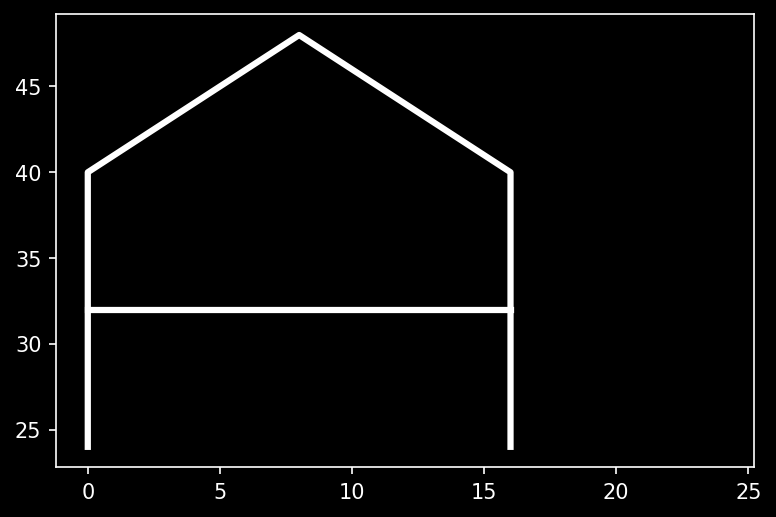
\includegraphics[width=12cm]{src/literals/A.png}%
    \end{adjustbox}
\end{figure}
\end{minipage}
\begin{minipage}[c]{0.48\linewidth}
\begin{lstlisting}[basicstyle=\scriptsize\ttfamily]
CHAR.A: VCTR 0,16,.BRITE
        VCTR 8,8,.BRITE
        VCTR 8,-8,.BRITE
        VCTR 0,-16,.BRITE
        VCTR -16,8,0
        VCTR 16,0,.BRITE
        VCTR 8,-8,0
        RTSL
\end{lstlisting}
\vspace*{\fill}
\end{minipage}

\begin{minipage}[c]{0.48\linewidth}
\begin{figure}[H]
    \centering
    \begin{adjustbox}{width=4cm,center}
      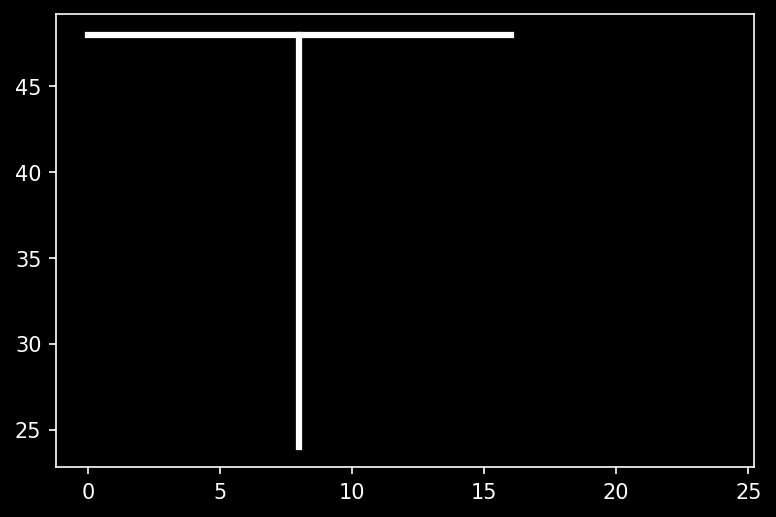
\includegraphics[width=12cm]{src/literals/T.png}%
    \end{adjustbox}
\end{figure}
\end{minipage}
\begin{minipage}[c]{0.48\linewidth}
\begin{lstlisting}[basicstyle=\scriptsize\ttfamily]
CHAR.T: VCTR 8,0,0
        VCTR 0,24,.BRITE
        VCTR -8,0,0
        VCTR 16,0,.BRITE
        VCTR 8,-24,0
        RTSL
\end{lstlisting}
\vspace*{\fill}
\end{minipage}

\begin{minipage}[c]{0.48\linewidth}
\begin{figure}[H]
    \centering
    \begin{adjustbox}{width=4cm,center}
      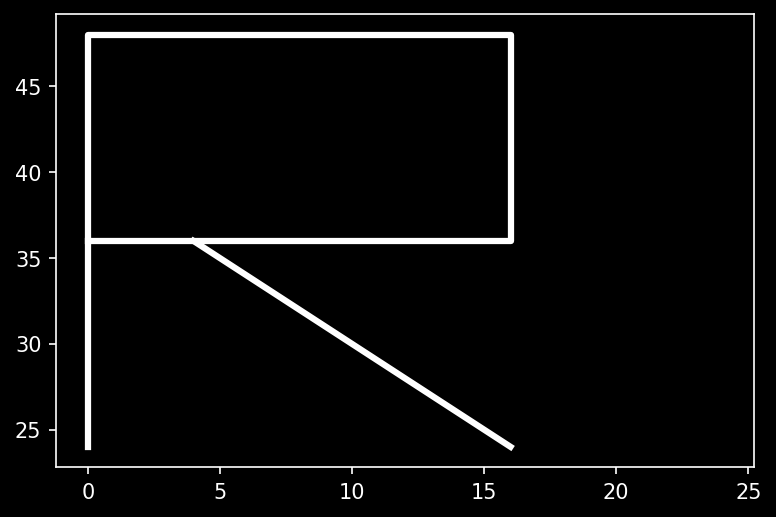
\includegraphics[width=12cm]{src/literals/R.png}%
    \end{adjustbox}
\end{figure}
\end{minipage}
\begin{minipage}[c]{0.48\linewidth}
\begin{lstlisting}[basicstyle=\scriptsize\ttfamily]
CHAR.R: VCTR 0,24,.BRITE
        VCTR 16,0,.BRITE
        VCTR 0,-12,.BRITE
        VCTR -16,0,.BRITE
        VCTR 4,0,0
        VCTR 12,-12,.BRITE
        VCTR 8,0,0
        RTSL
\end{lstlisting}
\vspace*{\fill}
\end{minipage}

\begin{minipage}[c]{0.48\linewidth}
\begin{figure}[H]
    \centering
    \begin{adjustbox}{width=4cm,center}
      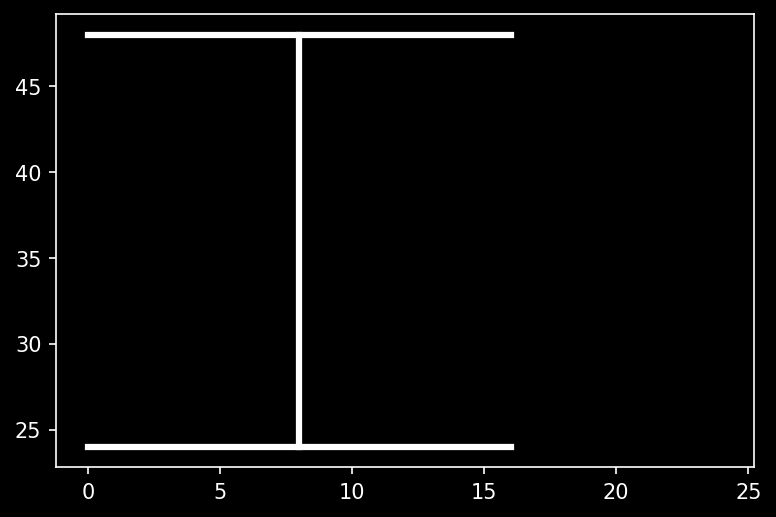
\includegraphics[width=12cm]{src/literals/I.png}%
    \end{adjustbox}
\end{figure}
\end{minipage}
\begin{minipage}[c]{0.48\linewidth}
\begin{lstlisting}[basicstyle=\scriptsize\ttfamily]
CHAR.I: VCTR 16,0,.BRITE
        VCTR -8,0,0
        VCTR 0,24,.BRITE
        VCTR 8,0,0
        VCTR -16,0,.BRITE
        VCTR 24,-24,0
        RTSL
\end{lstlisting}
\vspace*{\fill}
\end{minipage}

Nor is surprising that if we call them one after the other, in a particular order, that we might get the
anticipated result of drawing \icode{ATARI} to the screen:

\begin{minipage}[c]{0.48\linewidth}
\begin{figure}[H]
    \centering
    \begin{adjustbox}{width=4cm,center}
      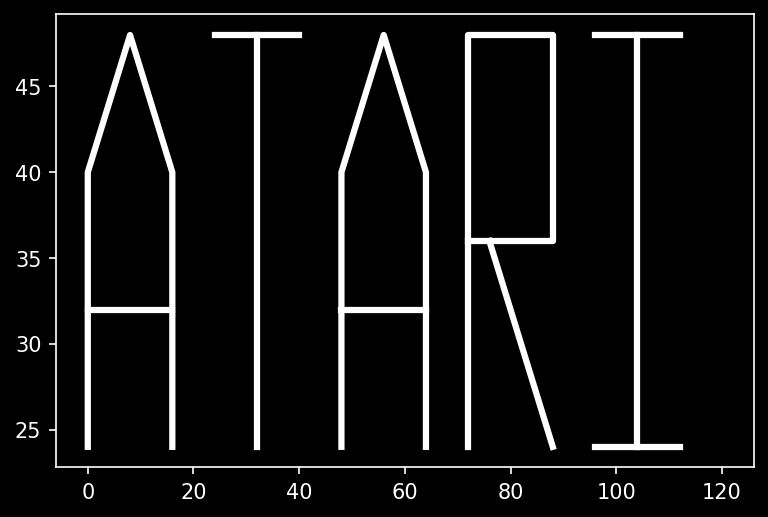
\includegraphics[width=12cm]{src/literals/atari.png}%
    \end{adjustbox}
\end{figure}
\end{minipage}
\begin{minipage}[c]{0.48\linewidth}
\begin{lstlisting}[basicstyle=\scriptsize\ttfamily]
JSRL    CHAR.A ; 36
JSRL    CHAR.T ; 1C
JSRL    CHAR.A ; 36
JSRL    CHAR.R ; 38
JSRL    CHAR.I ; A6 (16)
\end{lstlisting}
\vspace*{\fill}
\end{minipage}

So if we look for the piece of code responsible for using \icode{ASCVG} to write \textit{ATARI} to the
screen (as part of the copyright statement) we find this:
\begin{lstlisting}
EATARI:
FATARI:
GATARI:
SATARI:	ASCVH <^ MCMLXXX ATARI>
\end{lstlisting}
There appears to be an immediate catch, it is using something called \icode{ASCVH}
\footnote{Short for ASCii Vector Horizontal.}
rather than
the \icode{ASCVG} that we expected. But all is not lost, it turns out that \icode{ASCVH} is a
wrapper around \icode{ASCVG}. In addition to calling \icode{ASCVG} it first figures out the horizontal
position of the string. In fact, figuring out (and writing out) this horizontal position is
its sole function, apart from calling \icode{ASCVG} to write the string itself.

\begin{lstlisting}
  .MACRO ASCVH ...AR1,...AR2 ; MACRO ASCVH WITH 2 POSSIBLE ARGS.
  .NARG ...NUM               ; PUT NO. OF ARGS PASSED IN 'NUM'.
  .IF EQ ...NUM-1            ; IF ONLY THE STRING WAS PASSED..
  .NCHR ...HLO,<...AR1>      ; STORE THE NO. OF CHARS IN STRING IN 'HLO'.
  .BYTE -<...HLO*3>          ; HORIZONTAL POSITION IS HLO * 3.
  .ASCVG <...AR1>            ; CALL ASCVG TO WRITE OUT THE STRING.
  .IFF                       ; OTHERWISE POSITION AND STRING WERE PASSED..
  .BYTE ...AR1               ; SO OUTPUT ARG 1 AS THE HORIZONTAL POSITION
  .ASCVG <...AR2>            ; AND WRITE OUT THE STRING IN ARG 2.
  .ENDC                      ; END IF
  .ENDM                      ; END MACRO
\end{lstlisting}

\icode{ASCVH} can take two arguments: one for the horizontal position to draw the string,
and one for the string itself. If only one argument is passed, it assumes that its the string
and that it should display it in the horizontal center. This is the case with our current
example:

\begin{lstlisting}
EATARI:
FATARI:
GATARI:
SATARI:	ASCVH <^ MCMLXXX ATARI>
\end{lstlisting}

So we have managed to come quite far here: we have figure out how to draw text to the screen and
how to position it (horizontally) at least. But this still leaves a number of missing elements.
What about the vertical position? The color of the text? And most of all, what about writing
text in languages other than English? \icode{MCMLXXX ATARI} doesn't need translation, but messages
like \textit{'GAME OVER'} certainly do.  

So what we want is something to layer on top of \icode{ASCVH} that will give us all of the above
and produce a result that contains the vector instructions for writing all of our messages in all
of the languages that we're interested in.

To do this we have to think a little harder about the end result we want: lists of messages in all
four desired languages. This means we have to create four separate tables, one for each language.
And that each entry in each table should point to the message in that language. Since the position
on screen, color, and size is going to be common for each message, we can store that in a single,
separate table.

So we could imagine five tables in total, something like this:

\begin{figure}[H]
  {
    \setlength{\tabcolsep}{3.0pt}
    \setlength\cmidrulewidth{\heavyrulewidth} % Make cmidrule = 
    \begin{adjustbox}{width=12.5cm,center}
      \begin{tabular}{llllll}
        \toprule
        Message    &   \icode{ENGMSG} & \icode{FREMSG} & \icode{SPAMSG} & \icode{GERMSG} &  \icode{MSGLABS} \\
        \toprule
        GAME OVER & \icode{EGAMOV (012C)} & \icode{FGAMOV (0136)} & \icode{SGAMOV (0144)} & \icode{GGAMOV (014E)} & \icode{1C 9E} \\     
        PLAYER & \icode{EPLAYR (015E)} & \icode{FPLAYR (0166)} & \icode{SPLAYR(0166)} & \icode{GPLAYR (016E)} & \icode{80} \\     
        \copyright MCMLXXX ATARI & \icode{EATARI(0544)} & \icode{FATARI(0544)} & \icode{SATARI(0544)} & \icode{GATARI(0544)} & \icode{80} \\     
      \end{tabular}
    \end{adjustbox}
  }\caption*{The message tables. The pointer mnemonic, e.g. \icode{EGAMOV}, is a nickname for the hex address of the message, e.g. \icode(012C).}
\end{figure}

The key here is that for each message we have a separate table for each language, and each entry in the table
points to the instructions for drawing the string in that language. For words that require no translation,
the pointer will be to the same address. So in the case of \textit{\copyright MCMLXXX ATARI}, the entry
for each language points to the same address \icode{0544} in memory where the following
bytes are stored:

\begin{lstlisting}
EATARI:
FATARI:
GATARI:
SATARI:	
;  (C)   M  C  M  L  X  X  X     A  T  A  R  I
D3 50 00 2E 1A 2E 2C 44 44 44 00 16 3C 16 38 A6
\end{lstlisting}

You will hopefully recognize the bytes for 'ATARI' from earlier. As we discovered previously,
these are offsets into the alphabet table \icode{VGMSGA} that will draw each character.

An example where we actually have different messages for each language is \textit{GAME OVER}. For this we have a
different hex address in the entry for each language table, because we are pointing at a different message for 
each.
\begin{lstlisting}
EGAMOV:	ASCVH <GAME OVER>
FGAMOV:	ASCVH <FIN DE PARTIE>
GGAMOV:	ASCVH <SPIELENDE>
SGAMOV:	ASCVH <JUEGO TERMINADO>
\end{lstlisting}

So what we need is a way of adding these entries to the tables programatically, for example an instruction that
we can write as follows. One that will automatically add the \textit{GAME OVER} message to all four language tables
plus the table that defines the color, scale, and vertical position.

\begin{lstlisting}
MESS    GAMOV,GREEN,1,56   ; 'GAME OVER', COLOR, SCALE, VERTICAL POSITION.
\end{lstlisting}

Wouldn't it be great if this instruction created the first entry in each of our tables, 
at a stroke, like so:

\begin{figure}[H]
  {
    \setlength{\tabcolsep}{3.0pt}
    \setlength\cmidrulewidth{\heavyrulewidth} % Make cmidrule = 
    \begin{adjustbox}{width=12.5cm,center}
      \begin{tabular}{llllll}
        \toprule
        Message    &   \icode{ENGMSG} & \icode{FREMSG} & \icode{SPAMSG} & \icode{GERMSG} &  \icode{MSGLABS} \\
        \toprule
        GAME OVER & \icode{EGAMOV (012C)} & \icode{FGAMOV (0136)} & \icode{SGAMOV (0144)} & \icode{GGAMOV (014E)} & \icode{06 56} \\     
      \end{tabular}
    \end{adjustbox}
  }
\end{figure}

Well it turns out there is a macro we can write to do exactly that. It's called \icode{MESS}.
\footnote{Short for \textbf{MESS}age.}

\begin{lstlisting}
  .SBTTL  PREPARE TO MAKE MSG TABLES
  ; ARGS ARE: STRING, COLOUR, SCALE, Y-POSITION
  .MACRO MESS ...LIT,...COL,...SCA,...YPO ; START OF MACRO

  ; THE COMMENTS ASSUME WE HAVE PASSED GAMOV IN 'LIT'
  ; ADD ENTRY TO ENGMSG (ENGLISH TABLE)
  .=...ENG             ; POINT TO CURRENT POS IN ENGMSG
  .WORD E...LIT        ; ADD EGAMOV ('GAME OVER') TO ENGMSG.
  ...ENG=...ENG+2      ; MOVE CURRENT POS IN ENGMSG 2 BYTES FOR NEXT TIME.
    
  ; ADD ENTRY TO FRAMSG
  .=...FRE             ; POINT TO CURRENT POS IN FRAMSG
  .WORD F...LIT        ; ADD FGAMOV ('FIN DE PARTIE') TO FRAMSG.
  ...FRE=...FRE+2      ; MOVE CURRENT POS IN FRAMSG 2 BYTES FOR NEXT TIME.
    
  ; ADD ENTRY TO GERMSG
  .=...GER             ; POINT TO CURRENT POS IN GERMSG
  .WORD G...LIT        ; ADD GGAMOV ('SPIELENDE') TO GERMSG.
  ...GER=...GER+2      ; MOVE CURRENT POS IN GERMSG 2 BYTES FOR NEXT TIME.
    
  ; ADD ENTRY TO SPAMSG
  .=...SPA             ; POINT TO CURRENT POS IN SPAMSG
  .WORD S...LIT        ; ADD SGAMOV ('JUEGO TERMINADO') TO SPAMSG.
  ...SPA=...SPA+2      ; MOVE CURRENT POS IN SPAMSG 2 BYTES FOR NEXT TIME.
    
  ; ADD GLOBAL VARIABLE
M'...LIT=.MSNUM
  .GLOBL M...LIT       ; ADD GLOBAL VAR MGAMOV
  .MSNUM=.MSNUM+2
    
  ; ADD COLOR, SCALE, YPOS TO MSGLABS
  .=...CSY
  .BYTE <...COL*10>!...SCA  ; COLOR & SCALE ARE AND'D TOGETHER
  .BYTE ...YPO         ; AND Y POS IN A BYTE BY ITSELF.
  ...CSY=...CSY+2      ; MOVE CURRENT POS IN MSGLABS 2 BYTES FOR NEXT TIME.

  .ENDM                ; END OF MACRO
\end{lstlisting}

Notice some of the special behaviour available to the macro language here. We can take the literal
\icode{GAMOV} passed in the argument \icode{LIST} and manipulate it directly to reference each of
\icode{EGAMOV}, \icode{FGAMOV}, \icode{SGAMOV}, and \icode{GGAMOV}
individually. This allows us to output entries for each language table during assembly as though we had typed this:

\begin{minipage}[c]{0.23\linewidth}
\begin{lstlisting}[basicstyle=\scriptsize\ttfamily]
ENGMSG:
  .WORD EGAMOV
\end{lstlisting}
\end{minipage}
\hspace{0.2cm}
\begin{minipage}[c]{0.23\linewidth}
\begin{lstlisting}[basicstyle=\scriptsize\ttfamily]
FRAMSG:
  .WORD FGAMOV
\end{lstlisting}
\end{minipage}
\hspace{0.2cm}
\begin{minipage}[c]{0.23\linewidth}
\begin{lstlisting}[basicstyle=\scriptsize\ttfamily]
SPAMSG:
  .WORD SGAMOV
\end{lstlisting}
\end{minipage}
\hspace{0.2cm}
\begin{minipage}[c]{0.23\linewidth}
\begin{lstlisting}[basicstyle=\scriptsize\ttfamily]
GERMSG:
  .WORD GGAMOV
\end{lstlisting}
\end{minipage}

Because the macros are interpreted at assembly time and converted into machine language instructions,
this will make building our complete language tables a simple matter of issuing this instruction
for each message that we have defined:
\begin{lstlisting}
        .SBTTL  MESSAGES: COLOR, SCALE, Y POSITION, LANGUAGE PTRS
MESS    GAMOV,GREEN,1,56        ;GAME OVER
MESS    PLAYR,WHITE,0,1A        ;PLAYER (BIG)
MESS    PLYR2,WHITE,1,20        ;PLAYER (NORMAL)
MESS    PRESS,RED,1,56          ;PRESS START
MESS    PLAY,WHITE,1,38         ;PLAY
MESS    ENTER,RED,1,0B0         ;ENTER
MESS    PRMOV,TURQOI,1,0        ;SPIN
MESS    PRFIR,YELLOW,1,-10.     ;PRESS FIRE
MESS    HIGHS,RED,0,38          ;HIGH SCORE
MESS    RANK,RED,1,-50.         ;RANK
MESS    RATE,GREEN,1,10.        ;RATE YOURSELF
MESS    NOVIC,RED,1,-30.        ;NOVICE
MESS    EXPER,RED,1,-30.        ;EXPERT
MESS    BONUS,GREEN,1,-70.      ;BONUS
MESS    TIME,GREEN,1,98         ;TIME
MESS    LEVEL,GREEN,1,-40.      ;LEVEL
MESS    HOLE,GREEN,1,-55.       ;HOLE
MESS    INSER,RED,1,56          ;INSERT COINS
MESS    CMODE,GREEN,1,80        ;FREE PLAY
MESS    CMOD1,GREEN,1,80        ;1 COIN 2 PLAYS
MESS    CMOD2,GREEN,1,80        ;1 COIN 1 PLAY
MESS    CMOD3,GREEN,1,80        ;2 COINS 1 PLAY
MESS    ATARI,BLULET,1,92       ;MCMLXXX ATARI
MESS    CREDI,GREEN,1,80        ;CREDITS
MESS    BONPT,RED,1,0B0         ;BONUS PTS
MESS    2GAME,GREEN,1,89        ;2 GAME MINIMUM
MESS    BOLIF,TURQOI,1,89       ;BONUS EVERY
MESS    SPIKE,WHITE,0,0         ;AVOID SPIKES
MESS    APROA,BLULET,1,5A       ;APPROACH
MESS    SUPZA,BLULET,1,0A0      ;NEW SUPER
\end{lstlisting}

All of which will give us our four complete language tables.

\begin{minipage}[c]{0.23\linewidth}
\begin{lstlisting}[basicstyle=\scriptsize\ttfamily]
ENGMSG:
  .WORD EGAMOV
  .WORD EPLAYR
  .WORD EPLYR2
  .WORD EPRESS
  .WORD EPLAY
  .WORD EENTER
  .WORD EPRMOV
  .WORD EPRFIR
  .WORD EHIGHS
  .WORD ERANK
  .WORD ERATE
  .WORD ENOVIC
  .WORD EEXPER
  .WORD EBONUS
  .WORD ETIME
  .WORD ELEVEL
  .WORD EHOLE
  .WORD EINSER
  .WORD ECMODE
  .WORD ECMOD1
  .WORD ECMOD2
  .WORD ECMOD3
  .WORD EATARI
  .WORD ECREDI
  .WORD EBONPT
  .WORD E2GAME
  .WORD EBOLIF
  .WORD ESPIKE
  .WORD EAPROA
  .WORD ESUPZA
\end{lstlisting}
\end{minipage}
\hspace{0.2cm}
\begin{minipage}[c]{0.23\linewidth}
\begin{lstlisting}[basicstyle=\scriptsize\ttfamily]
FRAMSG:
  .WORD FGAMOV
  .WORD FPLAYR
  .WORD FPLYR2
  .WORD FPRESS
  .WORD FPLAY
  .WORD FENTER
  .WORD FPRMOV
  .WORD FPRFIR
  .WORD FHIGHS
  .WORD FRANK
  .WORD FRATE
  .WORD FNOVIC
  .WORD FEXPER
  .WORD FBONUS
  .WORD FTIME
  .WORD FLEVEL
  .WORD FHOLE
  .WORD FINSER
  .WORD FCMODE
  .WORD FCMOD1
  .WORD FCMOD2
  .WORD FCMOD3
  .WORD FATARI
  .WORD FCREDI
  .WORD FBONPT
  .WORD F2GAME
  .WORD FBOLIF
  .WORD FSPIKE
  .WORD FAPROA
  .WORD FSUPZA
\end{lstlisting}
\end{minipage}
\hspace{0.2cm}
\begin{minipage}[c]{0.23\linewidth}
\begin{lstlisting}[basicstyle=\scriptsize\ttfamily]
SPAMSG:
  .WORD SGAMOV
  .WORD SPLAYR
  .WORD SPLYR2
  .WORD SPRESS
  .WORD SPLAY
  .WORD SENTER
  .WORD SPRMOV
  .WORD SPRFIR
  .WORD SHIGHS
  .WORD SRANK
  .WORD SRATE
  .WORD SNOVIC
  .WORD SEXPER
  .WORD SBONUS
  .WORD STIME
  .WORD SLEVEL
  .WORD SHOLE
  .WORD SINSER
  .WORD SCMODE
  .WORD SCMOD1
  .WORD SCMOD2
  .WORD SCMOD3
  .WORD SATARI
  .WORD SCREDI
  .WORD SBONPT
  .WORD S2GAME
  .WORD SBOLIF
  .WORD SSPIKE
  .WORD SAPROA
  .WORD SSUPZA
\end{lstlisting}
\end{minipage}
\hspace{0.2cm}
\begin{minipage}[c]{0.23\linewidth}
\begin{lstlisting}[basicstyle=\scriptsize\ttfamily]
GERMSG:
  .WORD GGAMOV
  .WORD GPLAYR
  .WORD GPLYR2
  .WORD GPRESS
  .WORD GPLAY
  .WORD GENTER
  .WORD GPRMOV
  .WORD GPRFIR
  .WORD GHIGHS
  .WORD GRANK
  .WORD GRATE
  .WORD GNOVIC
  .WORD GEXPER
  .WORD GBONUS
  .WORD GTIME
  .WORD GLEVEL
  .WORD GHOLE
  .WORD GINSER
  .WORD GCMODE
  .WORD GCMOD1
  .WORD GCMOD2
  .WORD GCMOD3
  .WORD GATARI
  .WORD GCREDI
  .WORD GBONPT
  .WORD G2GAME
  .WORD GBOLIF
  .WORD GSPIKE
  .WORD GAPROA
  .WORD GSUPZA
\end{lstlisting}
\end{minipage}
